%!TEX program = xelatex
\documentclass[12pt,a4paper]{article}
% \documentclass[11pt,a4paper]{report}
% \documentclass[11pt,a4paper]{book}
% \def\mathfamilydefault{\rmdefault}

% 设置页面%==================================================
% \linespread{1}
%行距
% \headsep=2cm
% \textwidth=16cm\textheight=24.2cm
%==================================================

% 其它需要使用的宏包
%==================================================
\usepackage[UTF8,heading=true]{ctex}

\usepackage[colorlinks,linkcolor=blue,anchorcolor=red,citecolor=black,urlcolor=black]{hyperref}  \usepackage{tabularx}
\usepackage{authblk}                   % 作者信息
\usepackage{algorithm}                 % 算法排版
\usepackage{amsmath,amsthm,amssymb}               % 数学符号与公式
\usepackage{amsfonts}                  % 数学符号与字体
\usepackage{graphics}
\usepackage{accents}
\usepackage{color}
\usepackage{setspace}
\usepackage{cite}
\usepackage{changepage}
\usepackage[font=footnotesize]{caption}
\usepackage{fancyhdr}
\usepackage{fancyhdr}                  % 设置页眉页脚
\usepackage{fancyvrb}                  % 抄录环境
\usepackage{float}                     % 管理浮动体
\usepackage[top=3cm,bottom=3cm,left=2.5cm,right=2.5cm]{geometry}           % 定制页面格式
\usepackage{hyperref}                  % 为PDF文档创建超链接
\usepackage{lineno}                    % 生成行号
\usepackage{listings}                  % 插入程序源代码
\usepackage{multicol}                  % 多栏排版
\usepackage{natbib}                    % 管理文献引用
\usepackage{rotating}                  % 旋转文字,图形,表格
\usepackage{subfigure}                 % 排版子图形
\usepackage{titlesec}                  % 改变章节标题格式
\usepackage{moresize}                  % 更多字体大小
\usepackage{anysize}
\usepackage{indentfirst}               % 首段缩进
\usepackage{booktabs}                  % 使用\multicolumn
\usepackage{multirow}                  % 使用\multirow
\usepackage{graphicx}
\usepackage{xcolor}
\usepackage{titlesec}                  % 改变标题样式
\usepackage{enumitem}
\usepackage{parskip}
\usepackage[noend]{algpseudocode}
%==================================================

% 将默认的英文目录等改为中文,设置图号和公式号与章节对应,缩进大小
%==================================================
% \titleformat{\part}[display]{\centering\Huge}{\textbf{第~\thepart~部分}}{0.2cm}{\textbf}
% \titleformat{\chapter}[hang]{\huge}{\textbf{第~\thechapter~章}}{0.2cm}{\textbf}
% \renewcommand{\contentsname}{目 \quad 录}
% \renewcommand{\abstractname}{摘 \quad 要}
% \renewcommand{\appendixname}{附 \quad 录}
% \renewcommand{\theequation}{\arabic{section}.\arabic{equation}}      %公式号与章节对应
% \renewcommand{\figurename}{\normalsize{图 \arabic{section}.\arabic{figure}}}   %改figure为图
% \renewcommand{\refname}{参考文献}
% \renewcommand{\bibname}{参考文献}
% \makeatletter
% \renewcommand{\fnum@figure}[1]{\textbf{\figurename~}\hspace{10pt} \sffamily}   %图号与章节对应
% \makeatother\setlength{\parindent}{2em}       %设置缩进为两个大写M的宽度,大约为两个汉字的宽度
%==================================================

% 设置页眉页脚
%==================================================
% \renewcommand{\headrulewidth}{0.4pt}
% \renewcommand{\footrulewidth}{0.4pt}

% \pagestyle{headings}
% \pagestyle{fancy}
% \lhead{}
% \chead{}
% \rhead{}
% \lfoot{}
% \cfoot{}
% \rfoot{}
%==================================================

% 设置标题格式
%==================================================

\ctexset{
	section={
		%format用于设置章节标题全局格式,作用域为标题和编号
		%字号为二号,字体为宋体,左对齐
		%+号表示在原有格式下附加格式命令
		format+ = \zihao{3} \songti \raggedright,
		name={,\ },
		%beforeskip用于设置章节标题前的垂直间距
		%ex为当前字号下字母x的高度
		%基础高度为1.0ex,可以伸展到1.2ex,也可以收缩到0.8ex
		beforeskip = 1.0ex plus 0.2ex minus .2ex,
		%afterskip用于设置章节标题后的垂直间距
		afterskip = 1.0ex plus 0.2ex minus .2ex,
		%aftername用于控制编号和标题之间的格式
		%\hspace用于增加水平间距
		aftername = \hspace{0pt}
	},
	subsection={
		format+ = \zihao{-3} \songti \raggedright,
		name={,\ },
		%仅输出subsection编号且为中文
		beforeskip = 1.0ex plus 0.2ex minus .2ex,
		afterskip = 1.0ex plus 0.2ex minus .2ex,
		aftername = \hspace{0pt}
	},
	subsubsection={
		%设置对齐方式为居中对齐
		format+ = \zihao{4} \songti \raggedright,
		name={,\ },
		%仅输出subsubsection编号,格式为阿拉伯数字,打字机字体
		beforeskip = 1.0ex plus 0.2ex minus .2ex,
		afterskip = 1.0ex plus 0.2ex minus .2ex,
		aftername = \hspace{0pt}
	}
}

%==================================================

% 设置环境
%==================================================

\newenvironment{cnabstract}
{
{\songti \zihao{-4} \textbf{摘\ 要:}}
% 正文部分设置
\setlength{\baselineskip}{20pt} % 设置行间距为20磅
\songti % 宋体
\zihao{-4} % 小四
}

\newenvironment{keywords}
{
{\songti \zihao{-5} \textbf{关键词:}}
% 正文部分设置
\setlength{\baselineskip}{20pt} % 设置行间距为20磅
\songti % 宋体
\zihao{-5} % 小四
}

%==================================================

% 设置中文字体
%==================================================
%\setCJKmainfont[BoldFont=SimHei,ItalicFont=KaiTi]{SimSun}
\setCJKmainfont{SimSun}[AutoFakeBold]
%\setCJKmainfont[BoldFont={STHeiti}, ItalicFont={STKaiti}]{STSong}

%\setCJKsansfont{SimHei}
%\setCJKsansfont{Songti SC Regular}
%\setCJKsansfont{STHeiti}

%\setCJKmonofont{FangSong}
%\setCJKmonofont{Heiti SC Regular}
%\setCJKmonofont{STFangsong}

%-------------------------------------------------

\setCJKfamilyfont{zhsong}{SimSun}
% \setCJKfamilyfont{zhsong}{Adobe Song Std}
%\setCJKfamilyfont{zhsong}{STSong}

\setCJKfamilyfont{zhhei}{SimHei}
% \setCJKfamilyfont{zhhei}{Adobe Heiti Std}
%\setCJKfamilyfont{zhhei}{STHeiti}

%\setCJKfamilyfont{zhfs}{FangSong}
% \setCJKfamilyfont{zhfs}{Adobe FangSong Std}
%\setCJKfamilyfont{zhfs}{STSong}

%\setCJKfamilyfont{zhkai}{KaiTi}
% \setCJKfamilyfont{zhkai}{Adobe Kaiti Std}
%\setCJKfamilyfont{zhkai}{STKaiti}

%-------------------------------------------------

%\newcommand*{\songti}{\CJKfamily{zhsong}} % 宋体
%\newcommand*{\heiti}{\CJKfamily{zhhei}}   % 黑体
% \newcommand*{\kaishu}{\CJKfamily{zhkai}}  % 楷书
% \newcommand*{\fangsong}{\CJKfamily{zhfs}} % 仿宋

% !使用如下命令:{\songti 宋体} 可以临时使用宋体(要加大括号)
%==================================================

% 设置英文字体
%==================================================
%\defaultfontfeatures{Scale=MatchLowercase} % 这个参数保证 serif、sans-serif 和 monospace 字体在小写时大小匹配
% \setmainfont[Mapping=tex-text]{CMU Serif} % 使用 XeTeX 的 text-mapping 方案,正确显示 LaTeX 样式的双引号(`` '')
\setmainfont[Mapping=tex-text]{Times New Roman}
% \setsansfont[Mapping=tex-text]{CMU Sans Serif}
% \setsansfont[Mapping=tex-text]{DejaVu Sans YuanTi}
% \setmonofont{Courier New}
% \setmonofont{Monaco}
% \setmonofont{DejaVu Sans YuanTi}
%==================================================

% 题目,作者,日期
%==================================================
\title{\songti 年龄变换项目报告}

% Style 1
% -------------------------------

%\author[*]{\songti 李亦杨 10195101467}
%\affil[*]{\songti 10195101467}
%\author[**]{\songti 刁泽皓 10195101470}
%\affil[**]{\songti 10195101470}
% Style 2
% -------------------------------
%\author{\songti 李亦杨 10195101467}
%\affil{\songti \zihao{6} 10195101467}
%\author{\songti 刁泽皓 10195101470}
%\affil{affil2}
% Style 3
% -------------------------------
\author{
\songti
\begin{tabular}[t]{c c}
李亦杨 10195101467 & 刁泽皓 10195101470
\end{tabular}
}

\date{}
%==================================================


%%%%%%%%%%%%%%%%%%%%%%%%%%%%%%%%%%%%%%%%%%%%%%%%%%%
% 正文
%==================================================

\begin{document}
% \pagenumbering{Roman}          %页码为大写罗马数字
% \pagenumbering{arabic}         %页码为阿拉伯数字
\pagenumbering{gobble}

\setstretch{1}


\maketitle

% \newpage
% \tableofcontents

\pagestyle{empty}

\begin{adjustwidth}{0.5cm}{0.5cm}
	\begin{cnabstract}
		在此处输入中文摘要(字数一般不少于 500 字)。摘要必须反映全文中心内容,内容应包括目的、过程及方法、结论。要求论述简明、逻辑性强、尽量用短句。采用第三人称的写法,并请用过去时态叙述作者工作,用现在时态叙述作者结论。
	\end{cnabstract}
\end{adjustwidth}

\setlength{\parindent}{2em}
\setlength{\parskip}{0ex}

\section{生成对抗网络}
生成对抗神经网络(Generative Adversarial Networks)于2014年提出,其可以学习数据的分布规律,并创造出可以以假乱真的图像和文本。\textsuperscript{\cite{2014Generative}}


GAN的网络结构分为生成器和辨别器两部分。生成器读取一个随机的噪音输入,并输出一个图片,辨别器判别图片是否为训练集中的图片。当辨别器无法分辨真假(即判别正确的概率为$50\%$)时,训练结束。生成器和辨别器要分别搭建神经网络模型,可以根据实际需求选择卷积神经网络、递归神经网络或全连接神经网络。


GAN的模型训练过程可以大致概括为以下几个步骤:
\begin{enumerate}[itemindent=2em]
	\item 初始化生成器$G$和辨别器$D$两个网络的参数。
	\item 从训练集中抽取$n$个样本,同时让生成器利用定义的噪声$z$分布生成$n$个样本。固定生成器$G$,并训练辨别器$D$,使其尽可能区分真假。
	\item 循环更新$k$次辨别器$D$之后,更新$1$次生成器$G$,使辨别器尽可能地区分不了真假。
\end{enumerate}


在进行多次更新迭代后,理想状态下,只要最终辨别器$D$无法区分出图片到底是来自真实的训练样本集合,还是来自生成器$G$生成的样本即可。此时辨别的概率为$0.5$,完成训练。

迭代过程中的关键点在于损失价值函数的计算,Generative Adversarial Networks一文中提出了其计算公式\textsuperscript{\cite{2014Generative}}:
\begin{align}
	\underaccent{G}{min}\ \underaccent{D}{max}\ V(D, G) = \mathbb{E}_{x \sim p_{data}(x)}[log\ D(x)] + \mathbb{E}_{z \sim p_{z}(z)}[log(1-D(G(z)))]
\end{align}


其中真实数据$x$服从$p_{data}$分布,$p_{z}(z)$、$G(z)$是将噪音输入$z$映射到数据空间拟合真实图像后的分布,$D(x)$为得到真实数据(换言之,即辨别器无法分辨真假的数据)的概率。训练中需要取使得$D$最大的$x$分布,同时最小化伪造的概率$log(1-D(G(z)))$,以这一条件来训练生成器。

文章中严格证明了:
\begin{itemize}[itemindent=2em]
	\item 最优的生成器$G$存在满足$P_G=P_{data}$的唯一解,换言之当生成的图像分布与原数据分布近似的时候存在最优生成器。
	\item 最优辨别器需要满足$D(x)=\frac{P_{data}}{P_{data}+P_G}$,此时可以保证$V_(D,G)$能够取得唯一的极大值$0.5$。
	\item 只要有足够的训练数据和正确的环境,训练过程一定会收敛到最优。
\end{itemize}


\section{现行的主流年龄变化方案}
在Lifespan Age Transformation Synthesis之前,主流的年龄变化训练方案主要是为衰老的特定子因素建立单独的模型,其通常包含皱纹、纹理等代表性因素,同时着重于在离散的特定年龄下的转换。这些模型通常仅限于特定的域子集,即以风格或纹理差异为特征的同质域,换言之,这些转换常常基于风格迁移的思想。诸如DiscoGAN或CycleGAN一类的网络可以很好地完成这类图像翻译任务。在生成器部分,需要利用若干个卷积层构建编码器,用若干个卷积层构建解码器,同时在两者之间利用一个能够产生变化的深度网络来担当特征转换器。DiscoGAN使用CNN编码器和解码器,使用全连接网络当转换器,而CycleGAN则使用了ResNet充当转换器。\textsuperscript{\cite{2017Unpaired,2017Learning}}


基于此思路之上,基于CycleGAN实现的S2GAN在拟真性方面作出了改进,其通过抽象出身份信息,将个人的衰老基础以及传统年龄变换方案运用的群体化的特定年龄转变模式相结合,以生成具有个性化特征的人脸老化方案。S2GAN在编码器部分提取出个人的衰老模式作为个人特征,在解码器将人脸衰老特征解码,通过对几个年龄组进行加权得到目标图像,并在中间部分将线性组合系数与个人衰老特征相乘(而不是使用传统的连接)来完成年龄变化操作。\textsuperscript{\cite{2020S2GAN}}


然而以图像翻译作为年龄变换的主要思路,忽视了在年龄变化过程中头部发育带来的结构、形状变化,以及跨年龄段的外观变化问题。这也使得这些模型给出的年龄变换后的输出图像,相较于输入图像,往往只能呈现出在脸部各个子区域上的皮肤材质纹理(如皱纹)方面上的变化。


\section{另一种年龄变化方案}

\subsection{网络结构}
由与针对年龄转换这一应用场景,缺少捕捉人不同年龄段图像的大数据集,所以监督学习变得很困难,故转向对抗性学习,使用六个锚定的年龄类别来近似连续的老化过程,并提出了新的生成式神经网络结构。该网络由一个条件生成器和一个判别器组成,条件生成器负责跨年龄组的转换。


整个网络结构和训练过程如下图:


\begin{figure}[H]
	\centering
	\includegraphics[scale=0.7]{assets/layer_structure.png}
	\caption{网络架构}
\end{figure}


在预处理阶段,图像的背景和服饰元素通过使用相应的语义掩码被去除。年龄输入空间$Z$由一个$50*n$的向量组表示,其中$n$是年龄类别的数量,当输入年龄种类为$i$时,我们生成一个向量$z_i$:

\begin{align*}
	z_i\ =\ 1_i\ +\ v_i \quad v \sim N(0, 0.2^2 \cdot I)
\end{align*}

其中$1_i$是一个$50·n$元素向量,它包含元素$50·i$到$50·(i+1)-1$上的$1$和其他地方的$0$,$I$是单位矩阵。一个生成器被用来生成所有的目标年龄,它由三部分组成:身份编码器、潜在映射网络和解码器。训练过程中还使用了一个年龄编码器用来将真实和生成的图像嵌入年龄潜伏空间。


身份编码器$E_{id}$读取输入图像$x$并提取一个身份特征张量$w_{id}$,有$w_{id}=E_{id}(x)$。


映射网络$M:\ Z->W_{age}$,将年龄输入向量$Z$嵌入到统一的年龄潜在空间$Wage$。$M$是$8$层MLP网络,$Wage$是$256$元素的潜在向量。映射网络学习了最佳的年龄潜在空间,使之能够在年龄集群之间实现平滑的过渡和插值。


解码器读取年龄潜在编码和身份特征,并生成输出图像$y=F(w_{id},wage)$。其中身份特征$w_{id}$由样式化卷积块处理,为减少水滴伪影,模型将AdaIN归一化成替换为StyleGAN2中提出的调制卷积层,并且在每个调制卷积层后有一个像素范数层用来进一步减少伪影。


综上,从输入图像$x$和输入目标年龄向量$z_t$到输出图像$y$的整体生成器映射为:

\begin{align*}
	y\ =\ G(x,z_t)\ =\ F(E_{id}(x),M(z_t))
\end{align*}

年龄编码器将输入图像$x$映射到其在年龄向量空间$Z$中的正确位置。产生一个年龄向量$z_s=E_{age}(x)$,对应与图像$x$的源年龄簇$s$。
鉴别器,使用具有具有小批量标准偏差的 StyleGAN 鉴别器,并将最后一个全连接层修改为具有$n$个输出,以区分多个类别,对第$i$类的真实图像只会惩罚第$i$个输出。

\subsection{训练过程}
为了为了补偿年龄集群之间的不平衡,在每次训练迭代中,我们首先对源集群$s$和目标集群$t$进行采样,然后从每个类别中采样一张图片,执行三个前向传递:

\begin{align*}
	y_{gen}\ =\ G(x,z_t) \\
	y_{rec}\ =\ G(x,z_s) \\
	y_{cyc}\ =\ G(y_{gen},z_s)
\end{align*}

这里,$y_{gen}$是目标年龄$t$的生成图像,$y_{rec}$是源年龄$s$的重建图像,并应用一个循环从年龄$t$生成的图像$y_{gen}$重建源年龄$s$的$y_{cyc}$。 这些通道提供了所有必要的信号,以最小化以下损失函数,即:
\begin{enumerate}
	\item 对抗性损失
	\item 自我重建损失
	\item 循环损失
	\item 身份特征损失
	\item 年龄向量损失
\end{enumerate}

\section{代码实际运行结果}
由于设备原因,我们使用已经训练好的模型进行图像年龄转换。我们分别使用StarGAN(基于CycleGAN)与Lifespan Age Transformation Synthesis一文中提出网络,对S2GAN一文中使用的图片进行年龄转化.


原始图片如下:
\begin{figure}[H]
	\centering
	\includegraphics[scale=0.35]{assets/origin.png}
	\caption{原始图片}
\end{figure}


所得出的结果如下图:
\begin{figure}[H]
	\centering
	\includegraphics[scale=0.35]{assets/StarGAN.png}
	\caption{StarGAN,原始图片在最右侧}
\end{figure}


\begin{figure}[H]
	\centering
	\includegraphics[scale=0.35]{assets/S2GAN.png}
	\caption{S2GAN,原始图片在最左侧}
\end{figure}

\begin{figure}[H]
	\centering
	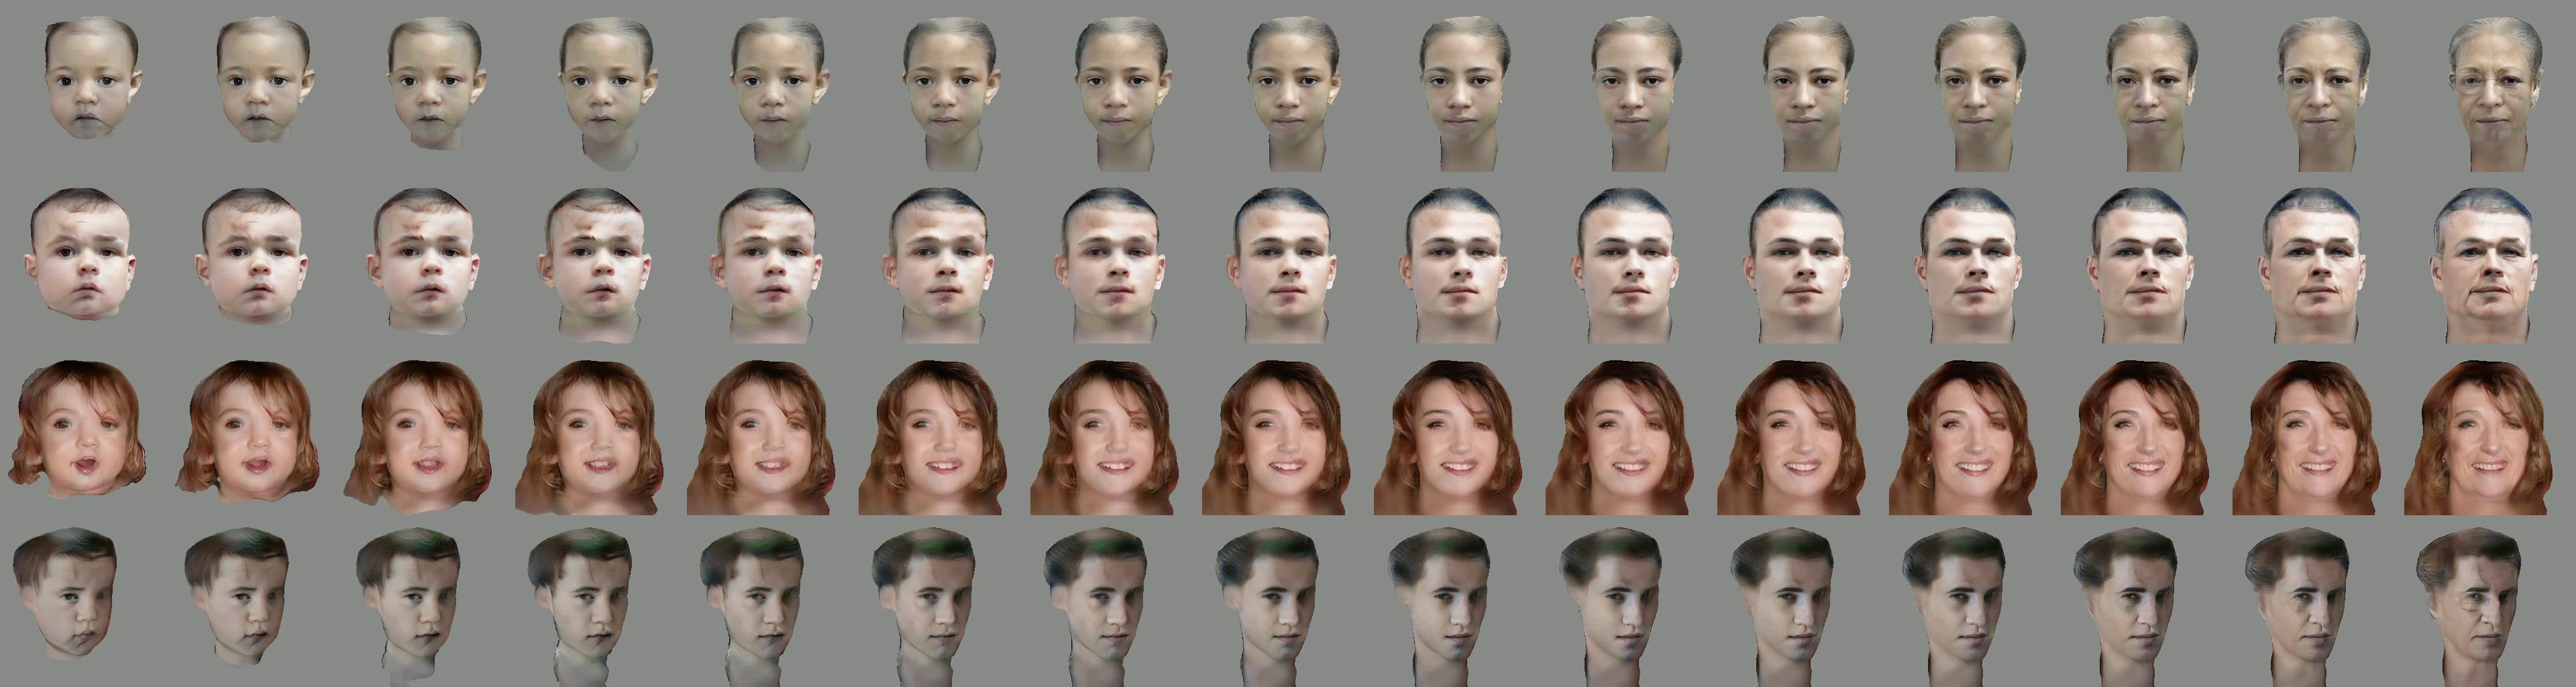
\includegraphics[scale=0.15]{assets/LATS.png}
	\caption{Lifespan Age Transformation Synthesis}
\end{figure}

可以发现,论文中提出的这一新模型在模拟年龄变化上具有更好的真实性,即人类成长过程中身体结构的变化也被考虑到了。然而,一些特定角度下的照片可能无法较好地模拟,同时一些纹理上的表现可能有所不足。


\bibliographystyle{unsrt}
\bibliography{main}



% \newpage

\end{document}
%==================================================
%%%%%%%%%%%%%%%%%%%%%%%%%%%%%%%%%%%%%%%%%%%%%%%%%%%
